\documentclass{beamer}
\usepackage[utf8]{inputenc}
\usepackage{lmodern}
\usepackage{bookmark}
\usepackage{graphicx}
\usepackage{xeCJK} %导入中文包
\setCJKmainfont{SimHei} %中文字体采用黑体  Microsoft YaHei
\usetheme{Hannover}
\usecolortheme{spruce}
\tiny
\title{Graph Convolutional Network}
\author{josephlin}

\begin{document}

\frame{Graph Convolutional Network}

\section{Introduction}
\begin{frame}
    \frametitle{CNN}
    CNN中的卷积本质上就是利用一个共享参数的过滤器(kernel),通过计算中心像素点以及相邻像素点的加权和来构成feature map实现空间特征的提取,当然加权系数就是卷积核的权重系数。卷积核的系数通过是随机化初值,然后根据误差函数通过反向传播梯度下降进行迭代优化。\\
    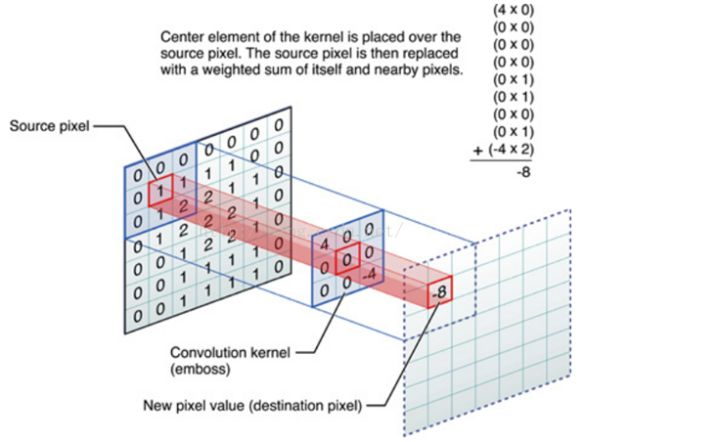
\includegraphics[height=4cm]{images/feature_map.jpg}
\end{frame}

\begin{frame}
    \frametitle{CNN}
    CNN处理的图像或者视频数据中像素点(pixel)是排列成成很整齐的矩阵。\\
    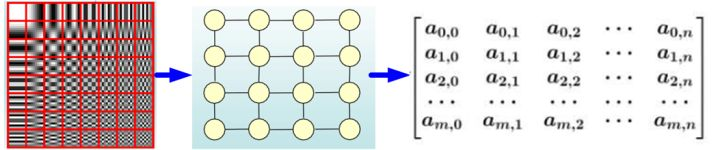
\includegraphics[height=2cm]{images/Euclidean_Structure.jpg}\\
    科学研究中还有很多Non Euclidean Structure的数据,GCN用以处理 Non Euclidean Structure 结构矩阵
    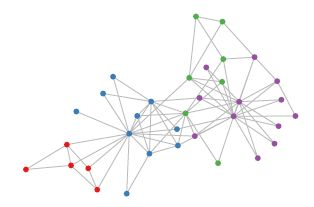
\includegraphics[height=2cm]{images/Non_Eclidean_Structure.jpg}
\end{frame}

\section{Model}
\begin{frame}
    \frametitle{Notation and Problem Statement}
    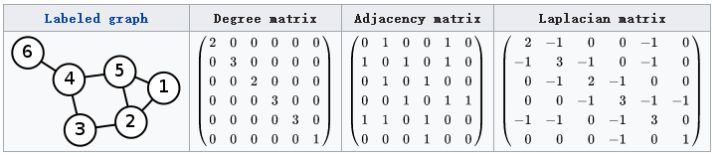
\includegraphics[height=2cm, width=10cm]{images/laplacian.jpg}\\
    对于图$G=(V, E)$,其Laplacian矩阵的定义为$L=D-A$,其中$L$是Laplacian矩阵,$D$是顶点的度矩阵(对角矩阵),对角线上元素依次为各个顶点的度,$A$是图的邻接矩阵。

\end{frame}

\begin{frame}
    \frametitle{谱分解}
    对拉普拉斯矩阵进行谱分解(特征分解)\\
    $$L= U\left(\begin{matrix}\lambda_1 & \\&\ddots \\ &&\lambda_n \end{matrix}\right) U^{-1}$$\\
    拉普拉斯矩阵是半正定对称矩阵,故其特征向量构成的矩阵为正交矩阵($UU^{T}=E$)\\
    $$L= U\left(\begin{matrix}\lambda_1 & \\&\ddots \\ &&\lambda_n \end{matrix}\right) U^{T}$$

\end{frame}

\begin{frame}
    \frametitle{傅立叶变换}
    
\end{frame}

\end{document}